\chapter[A$\beta$42]{Molecular Mechanism of A$\beta$42 fibril inhibition by inositol}

% Some notes
% I found these pretty neat ref articles on sciencedirect
% http://www.sciencedirect.com.myaccess.library.utoronto.ca/science/article/pii/B9780444519672001550
% http://www.sciencedirect.com.myaccess.library.utoronto.ca/science/article/pii/B9780444519672000581
% http://www.sciencedirect.com.myaccess.library.utoronto.ca/science/article/pii/B9780444519672000313
% http://www.sciencedirect.com.myaccess.library.utoronto.ca/science/article/pii/B0080437486011592

	
\section{Summary}
Alzheimer's disease (AD) is a severe neurodegenerative disease with no cure. Currently, one method of targeting the underlying disease is to prevent or reverse the amyloid formation of A$\beta$42, a key pathological hallmark of AD. A small-molecule novel drug candidate, Scyllo-inositol, is a polyol small-molecule that exhibits stereochemistry dependent inhibition of the formation of fibrils in vitro.  Furthermore, recently completed phase II clinical trials demonstrated that scyllo-inositol achieved target drug levels in the cerebral spinal fluid (CSF) of AD patients, a main challenge for AD drug candidates to to overcome.

Despite its promise as a therapeutic for AD, the mechanism of action of scyllo-inositol at the molecular level is currently not understood.  We perform extensive atomistic molecular dynamics simulations of scyllo-inositol and its inactive stereoisomer, chiro-inositol, glucose, and the osmolyte protein stabilizer, glycerol, with the full length A$\beta$42 protofibril.  From our simulations, we characterize the stereochemistry-dependent binding modes of these three cosolu on the structure of A$\beta$42 protofibrils.  Our results provide molecular insight for the rational design of small-molecule inhibitors of A$\beta$42 and other amyloid-based diseases.

  \textbf{Keywords}:
	amyloid computational
	amyloid inhibition
	small molecule amyloid inhibition
	amyloid disaggregation
	inositol
	surface binding
	weak interactions
	carbohydrate like interactions

\section{Introduction}

% Why Abeta42 
\abeta42 is the pathological hallmark of Alzheimer's Disease (AD) and forms the largest proteinaeous component of plaques in the brain of AD patients. \abeta\ peptides are produced from the cleavage of amyloid precursor protein (APP) in isoforms with lengths of 33 to 42 residues. Although \abeta42\ and \abeta40\  peptides differ in length only by two residues, they have a number of notable differences: \abeta42\ is found to display significantly higher aggregation propensity\cite{Jarrett:1993vm,Fukumoto:1996vi,Finder:2010jw} and cellular toxicity than \abeta40\ peptides.\cite{ElAgnaf:2000hp,Mucke:2000uqa}  Furthermore, they are found to form fibrils via distinct pathways.\cite{Bitan:2003ut,Sanchez:2011bj,Bitan:2003p1781}
% This difference in the two residues confer significant differences in their aggregation propensity and toxicity.
% Do I really need to talk about polymorphism?
% Although the \crossbs\ is the core tertiary structure found for all amyloid fibrils, fibrils exhibit polymorphism at the residue-level depending on their formation conditions.\cite{Wu:2010p3553} \textbf{where they different polymorphs?} Different amyloid fibril structures may exhibit different toxicities.\cite{Paravastu:2009fi,Wu:2010p3553}
% Fibril structures of \abeta40\ and \abeta42\ were also found to be similar.\cite{Wu:2010p3553} There are brain derived structures of \abeta40, their structures are different from the synthetic ones because of polymorphism. 


% Rationale for studying the Abeta42 protofibril system	-- there is all this abeta40 stuff simply because its easier to work with these peptides, but then abeta42 is the actual important peptide that people should be looking at!
In the past few years, many studies have probed the aggregation properties of \abeta40. Fibril models of the \abeta40\ peptide derived from solid-state NMR (SSNMR) indicate that protofilaments of \abeta40\ contain 2 to 3 layers.\cite{Wu:2010p3553,Tycko:2010iz} By contrast, much less is known about the fibril structure of \abeta42. A SSNMR model of the fibril of \abeta42\ was recently proposed by Luhrs et al. In that model, N-terminus of \abeta42\ in the fibril was found to be unstructured.\cite{Ahmed:2010p5694} A previous MD simulation study of \abeta42\ protofibrils in pure water suggests that residues 17 to 42 are predominantly involved in the stability of the core structure of the fibril.\cite{Masman:2009p6410}

% \textbf{Small molecules are promising candidates for the treatment of AD. Many of them have been found to display anti-aggregation activity, including osmolytes.} 
In recent years, drug development and research efforts have been directed towards the development of therapeutic agents to prevent the self-aggregation and amyloid formation of A$\beta$, a promising treatment approach to target the underlying disease.\cite{Masters:2006p183,Citron:2010p214,Dasilva:2010p25} As a result, many different types of \emph{in vitro} amyloid inhibitors have been discovered, including peptides,\cite{EsterasChopo:2008p219,Sciarretta:2006p181,Chalifour:2003p161,Scrocchi:2002p178,Soto:2007dm} immunotherapies,\cite{Janus:2000p198,Solomon:2010p177} polyphenolic molecules,\cite{Masuda:2009p205,Berhanu:2010p230,Ehrnhoefer:2008p8} and other small molecules.\cite{Hawkes:2009p189,Masuda:2009p205,Necula:2007p227,Nitz:2008p13} These approaches have been reviewed in detail elsewhere.\cite{Citron:2010p214,Dasilva:2010p25}

\emph{scyllo}-Inositol is a small-molecule inhibitor of A$\beta$42-fibrillation developed for the treatment of AD.\cite{McLaurin:2006p29,McLaurin:2000p64,Fenili:2007p182,Ma:2012jk} 
Inositol is a class of cyclohexylpolyols, of which eight out of nine stereoisomers are commonly found in nature. \emph{scyllo}-Inositol, with all hydroxyl groups equatorial,  is the only isomer with two planar hydrophobic faces. By contrast, its diastereisomer, \emph{chiro}-inositol, with two adjacent axial hydroxyl groups, has two nonplanar  hydrophobic faces.  Importantly, \emph{scyllo}-inositol was demonstrated to prevent and reverse AD-like symptoms in a transgenic mouse model of AD.\cite{McLaurin:2006p29} Because of the positive CNS bioavailability and favorable \emph{in vivo} toxicity profile of inositol, both of which are rare and essential properties of putative AD drug candidates, inositol-based therapies represent unique and promising approach for the treatment of AD. Phase II of clinical trials for \emph{scyllo}-inositol (ELN0005) in North America was fast-tracked in 2007 by the United States Food and Drug Administration and was completed in 2011.\cite{Salloway:2011im,Ma:2012jk}

\emph{In vitro}, inositol displays stereochemistry-dependent inhibition of A$\beta$42 fibrils: \emph{scyllo}-inositol was shown to inhibit A$\beta$42 fibrillation at concentrations of 1 - 5 mM,\cite{McLaurin:2000p64} whereas \emph{chiro}-inositol is inactive below molar concentrations.\cite{Janus:2000p198} Moreover, upon incubation of monomeric A$\beta$42 with \emph{scyllo}-inositol, circular dichroism spectroscopy indicated the formation of $\beta$-sheet structure at an inositol:peptide molar ratio of 25:1.\cite{McLaurin:1998p176} 

Although inositol stereoisomers have been proposed to inhibit amyloid formation by directly interacting with either monomers or non-fibrillar aggregates to ``cap off'' fibril growth,\cite{Janus:2000p198} the molecular basis of the effect of \emph{scyllo}-inositol and its stereoisomers on A$\beta$42 amyloid formation is currently unknown.
% \cite{Nikolic:2011p185,Rauscher:2006p43,Li:2012p853,Rauscher:2010p5682,Sgourakis:2011hy,Wang:2005do,Cino:2011ff}

Organic osmolytes (e.g., TMAO, glycerol, glucose) are small molecules that stabilize the folded state of proteins. Examples include TMAO, glycerol, and are thought to do so via the preferential exclusion mechanism.\cite{Bolen:2001im}  In recent years, osmolyte, small molecules which stabilize the folded state of proteins, have been found to modulate amyloid formation\cite{Sukenik:2012dv,Sukenik:2011p8778}. TMAO,\cite{Seeliger:2013cj}betaine,\cite{Natalello:2009fn} glucose,\cite{Fung:2005p2008} trehalose\cite{Nayak:2009fr} and glycerol\cite{Sukenik:2011p8778} been found to modulate amyloid formation and peptide aggregation.\cite{Liu:2005km,Sukenik:2011p8778,Fung:2005p2008}
% In particular, glycerol is able to slow the kinetics of fibrillation (I don't think this is correct -- check this again).\cite{Yang:1999ws}This paper did a study on myo-inositol, but from a fast scan I wasn't able to figure out what their conclusions for myo- and other polyols are.\cite{Macchi:2012ci}

Molecular dynamics (MD) simulations are well-suited for studies of disordered proteins and can provide atomic-level insight into the mechanism of inhibition of peptide self-aggregation by small molecules. MD simulations were previously employed to examine the binding mechanism of other small-molecule inhibitors such as polyphenols,\cite{Lemkul:2010p23,Wang:2010p204} non-steroidal anti-inflammatory drugs\cite{Raman:2009p47,Takeda:2010p34}, and the well-known amyloid dye thioflavin T\cite{Wu:2008ds,Wu:2011fd} to monomers and/or fibrillar forms of A$\beta$\cite{Liu:2009p213}. 

Because of the existence of multiple aggregation states, small-molecule inhibitors may have multiple modes of action and may act by binding either to monomers\cite{Ehrnhoefer:2008fd} or to non-fibrillar or fibrillar oligomers\cite{Buell:2010p9457} in the fibrillation pathway. Furthermore, their inhibitory activity may also be affected both by the concentration of the ligand and by the ligand:peptide molar ratio.\cite{Wang:2010p204,LeVine:2005cv}  

% However, thus far, few MD simulation studies have examined the effect of ligand concentration on different relevant aggregation states along the amyloid fibrillation pathway.\cite{Wang:2010p204}

% \textbf{Do I need this? Say why its important to look at binding for Abeta42 instead}
% On the basis of current high-resolution structural data, there are several differences between the fibril structures of A$\beta$42 and A$\beta$40.\cite{Ahmed:2010p5694} \textbf{ADD: what are their differences}

% In recent years, scyllo-inositol, a small-molecule polyol, has demonstrated promise as a potential therapeutic of Alzheimer's Disease. scyllo-inositol displays stereochemistry-dependent activity of amyloid inhibition of \abeta42.REF In studies with a mouse model of AD, scyllo-inositol was shown to prevent and reverse the on-set of AD.REF 

% Where would this idea fit? Small-molecule modulators of amyloid formation may be classified into those that accelerate and / or stabilize amyloid formation and those that displace the equilibrium towards the disaggregated state (inhibitors of amyloid formation).

In two previous studies, using MD simulations, we successively examined the binding mechanism of scyllo- and chiro-inositol with peptide and aggregate states of model amyloid-forming peptides and A$\beta$(16-22), the central hydrophobic core of A$\beta$. Weak and stereochemistry independent binding of inositol with the peptidic backbone was found, with binding constants in the range of 0.1 - 1 M, indicating that inositol is unlikely to inhibit amyloid formation by binding the peptidic backbone alone.\cite{inos1} However, in our study involving A$\beta$(16-22), inositol was found to preferentially bind to the surface of $\beta$-sheet oligomers, but only weakly to those of disordered or monomeric forms. Furthermore, inositol was found to adopt cooperative, high avidity binding modes with $\beta$-oligomers with binding constants commensurate with the \emph{in vitro} inhibitory concentrations.  Taken together, the results from our previous studies indicate that inositol is likely to disrupt amyloid fibrillation by binding to  $\beta$-sheet oligomers of A$\beta$.

\textbf{Need a lot more detail here} In this study, we examine the binding mechanism of inositol stereoisomers, scyllo- and chiro-inositol, along with glucose and glycerol, with the SSNMR model protofibril of the full-length \abeta42.  Both glucose and glycerol affect fibrillation of A$\beta$42\ at concentrations of more than 1 M. Our results provide insight into the structure-activity relationship of inositol in the inhibition of A$\beta$ amyloid formation, which will ultimately lead to forming a pharmcophore for treating AD and related neurodegenerative disorders.

% For now, I removed the table of simulations.  There is no variation in the system run times or molar ratio. Can just mention this or put this table in supplementary information.
  
\section{Material and Methods} % (fold)
\label{sec:material_and_methods}

The pentameric solid-state NMR model of A$\beta$(17-42) from Luhrs et al. (PDB code: 2BEG) was used as the starting structure in our simulations.\cite{Luhrs:2005p4900} In the PDB structure, residues 1 to 16 were truncated in the model because they are disordered.\cite{Luhrs:2005p4900} Because the truncation at the N-terminal ends of the peptides is artificial,  acetyl groups to the peptides, yielding an uncharged N-terminal end of the fibril. The acetyl groups were modeled onto the fibril using PyMol. Titratable amino acids were assigned charged states at the physiological pH. 10 sodium ions were added neutralize the remaining charges in the system. To mimic experimental conditions, 0.15 M of salt were added. Protein and solvent were represented by the OPLS-AA/L force field\cite{Jorgensen:1996vx} and the TIP3P water model,\cite{Jorgensen:1983p8768} respectively.  The  extended OPLS-AA force field for carbohydrates was used to model inositol stereoisomers and glucose.\cite{Damm:1997tla}

All MD simulations were performed in the NpT ensemble using the GROMACS simulation package version 4.0.x.\cite{Hess:2008p5353} The leapfrog Verlet integration algorithm was used with an integration timestep of 2 femtoseconds. Long-range electrostatic interactions were calculated using Particle Mesh Ewald (PME) summation with a Fourier grid spacing of 0.15 nm and a real-space cutoff of 1.3 nm.\cite{Darden:1993p8963} The short-range nonbonded van der Waals interactions were switched to zero from 1.1 nm to 1.2 nm. The temperature was controlled at 300 K using the Nose-Hoover thermostat. Pressure was controlled by the Parrinello-Rahman barostat at 1 atm with a coupling constant of 4.0 ps. The SHAKE algorithm was used to constrain covalent bonds containing hydrogens.\cite{Ryckaert:1977p9357}

In all simulations, a cubic box was used and periodic boundary conditions. Prior to data collection, 500 steps of energy minimization using the conjugate gradient algorithm was first performed, followed by a 200 ps long equilibration in the NVT ensemble and a 2 ns long equilibration with isotropic pressure coupling (NPT ensemble). The center of mass (COM) rotation and translation were removed at every step.

A set of ten 0.250 $\mu$s simulations of the protofibril of \abeta42 were performed,  successively, in pure water and in the presence of scyllo-inositol, chiro-inositol, glycerol and glucose. The ligands were present at either a ligand:peptide molar ratio of  15:5 or 64:5, yielding a total sampling time of 12.5 $\mu$s.

\subsection{Analysis Protocol}
GROMACS analysis tools g\_rmsd and g\_rmsf were used to calculate the root mean square deviation in the fibril backbone and root mean squared fluctuation, respectively.  Spatial probability density of bound inositol were calculated using the volmap tool in Visual Molecular Dynamics software package (VMD). 

Nonpolar contacts between inositol and fibril were defined by a carbon to carbon cutoff of 0.X nm. The DSSP hydrogen bonding criteria were used to determine the existence of a hydrogen bond.  Secondary structure analysis was performed using do\_dssp using the DSSP algorithm.

Interchain hydrogen bonds (s1 - s2, s2 - s3, s3 - s4, s4 - s5) were computed between adjacent strands in the fibril using g\_hbond.  Hydrogen bonding criteria used acceptor-donor heavy atoms with distance less than 0.35 nm and hydrogen-donor-acceptor angle of less than 30 degrees (CHECK THIS).
	
% Contact map of inositol to A$\beta$42
Binding constants are calculated by assuming the reaction,

% Equations used in the KLVFFAE paper
\[ \left[ Protein\cdot Inositol \right] \rightleftharpoons \left[ Protein \right] +\left[ Inositol \right] \]

Where,

\[ K_{d} = f_{ub}\frac{\left[ Protein \right]\left[ Inositol \right]}{\left[Protein \cdot Inositol\right]} \]

% Equation converting population to free energy
% $\mathit{W}=-RT\ln\rho\left(r,\theta\right)$
% $\rho\left(r,\theta\right)$

\section{Results}

\subsection{Protofibrillar morphology}
Here I can show the RMSF and RMSD and the secondary structure information.  The point is to show that the protofibril stays in tact or not.  If intact, then say that it did not break up the protofibril on the timescale of our simulations.

The technical details involve getting all this data into a columnar form.  First plot the curves separately to identity outliers if any and see why they've deviated by looking at the trajectories for making further hypothesis.

\subsection{Comparisons of scyllo, chiro, glycerol and glucose binding modes}
Which residues most frequently bound \\

Over all binding modes.  Use the spatial probability maps to demonstrate this \\
Are there binding hot spots? If so where and what are they? [in the discussion relate these findings to the mechanism of amyloid formation]

Mostly nonpolar or polar? \\

Do the molecules Cluster? If so, do cluster sizes differ? For example do glycerol and glucose  cluster a lot less? If there are differences in this mechanism could have implications in the mechanism of amyloid formation. \\

How do the results compare with my previous results [discussion?] \\

Does any of these molecules target the fibril core? [discussion?] \\
Is targeting the fibril core a plausible mechanism for breaking up amyloid fibrils? Address this. Previous studies don't really address them.  
In the discussion, I think it will also help to have a comparisons with previous studies, and experimental studies, if applicable. Again, look into literature for updates.




%\begin{itemize*}
%	\item The fibril morphology in their presence.  There is only a subtle difference (really? what is this difference? I think I want to retract this statement)
%	\item Does glycerol stabilize the aggregate? Does glucose stabilize the fibril?
%	\item Is the protofibril equally stable in water and in inositol?
%\end{itemize*}
%
%\subsubsection{Inositol and cosolvent Binding} % (fold)
%\label{sub:subsection_name}
%\begin{itemize*}
%
%	\item Global binding
%	\begin{itemize}
%		\item Spatial distribution of bound inositol
%		\item From a single spatial distribution density for scyllo and chiro-inositol, chiro-inositol bound and passed through the intersheet channel in the fibril, where as scyllo appear to be trapped at the entrance and does not move through the \"channel\". Note that a recent paper by Shea et al. also demonstrated this with dye molecules.	
%		\item Contact map -- needed? Yes I think I should further quantitate their binding mode differences. Just by looking at the spatial maps, the differences are minor and need a trained eye.  Having a contact map by residue will be more rigorous. Also quantitate binding affinity per binding pocket. This helps define binding sites on the fibril more precisely. Overall I have more binding statistics than all of the other relevant studies out there, I should take advantage of this. The global binding modes suggests that the active ligand, scyllo-inositol is able to bind the KLVFFAE face better. I need to relate this to fibril inhibition. Furthermore, all of my models are converging on similar answers (that is binding to protofibrils, and binding to KLVFFAE segment), which is reassuring!
%	\end{itemize}
%
%	\item Does inositol, glucose and glycerol, preferentially partition to different areas of the protofibrillar surface? Based on the global binding mode as shown in the spatial distribution, the answer to this is yes. But it would be really cool to know the nonpolar and polar binding modes for each of these (that is the pie charts). If there is a difference, I can then extrapolate and correlate these differences to the SAR of inositol.
%	
%	\begin{itemize}
%		\item Nonpolar contacts 
%		\item Polar contacts
%		\item Binding constants - How do I calculate this?  Inositol never fully dissociates (when saturated) so, in this case, it is more of a residence time in the binding pocket(s). Yes calculate the residence time!  Hmm how do I calculate the residence time? This would link up with the binding kinetics.
%	\end{itemize}
%\end{itemize*}
%
%
\section{Discussion}
%Comparisons to earlier simulation studies of inhibitor binding to A$\beta$42 and A$\beta$40 relevance of the NMR models.
%``accuracy'' of the NMR models -- how good are these models?  It is unlikely I'm going to be able to say much here, we have no idea what the actual experimental stability of this species is.  This pentamer fragment may not be stable on its own, but could be just a building block in a stable extended fibrillar structure of A$\beta$42.
%
%% look into literature here, read a bit, and critically summarize and fit into the context of my work.
%% April 17th 
%% Recent papers
%% Shea and Bower 2012 in Biochemistry - They looked at CTF binding to Abeta40 and 42 both experimentally and using simulations.  The data here is not that quantitative, esp. the simulation data.  Suggest that N-terminal part of Abeta42 is more responsible for toxicity than the C-termininal.  Also CTF binds at N-terminal (which residues? Don't think this data was in their paper). Does it include 16-22 fragments?
%% Abelein et al..Dobson 2012 - Lacmoid binding to Abeta40 and Abeta42.  
%% - Proposes a similar mechanism that I am proposing in my KLVFFAE paper .. however they find that Lacmoid most likely binds to the monomer, and in a surfactant-like manner (I think this corresponds to what I call "coating"). 
%% - Makes ample references to a paper by Otzen DE http://www.ncbi.nlm.nih.gov/pubmed/20423296 on amyloid aggregation induced by surfactants.  Might be useful to read up on surfactants, micelle formation and what the field knows there.  I can be sure that there will be analogies drawn to this field in my thesis defense.
%% - I like what they wrote in the discussion to interpret their data as it somewhat supports my findings, but again speculative and results are STILL pretty qualitative.  
%% - Note that this paper might be useful for Aditi to look at ... could she reuse / use some of their protocols?
%
%\subsection{Solute binding}
%
%\begin{itemize}
%	\item 	Different binding modes between scyllo and chiro-inositol
%	\begin{itemize}
%		\item From a single spatial distribution for scyllo and chiro, I did not see scyllo go all the way through the “channel”, where as chiro does! (RESULT)
%		\item Is this true in general? Perhaps this is a reason why scyllo works better?  - More specific interactions? ie.  Chiro just gets trapped in ``non-productive'' binding modes.
%			\begin{itemize}
%				\item Note that Shea also observes this in her paper.\cite{Wu:2011fd}
%			\end{itemize}
%	\end{itemize}
%	\item Sugar binding to the A$\beta$42 fibril -- appears to stabilize? I don't think so … this isn't true from looking at the data.
%	
%	\item Inositol interestingly also seem to binding similarly to guanidinium ions around a hydrophobic surface. (Personal communication with Shekhar - Said to me during CBP that they see similar results from their guanidinium ion studies ... what does this really mean?)
%	
%	\item How does binding differ from binding to KLVFFAE, a small fragment of A$\beta$42 ?  Inositol partition differently depending on the sequence. 
%	\begin{itemize}
%		
%		\item Comment on how good are these model peptides for understanding inhibitor binding interactions. Do I really want to discuss this? Depending on the model (the protofibril), the binding modes can be different depending on the aggregate morphology as we've shown in our earlier studies. In our previous study, we examined binding with KLVFFAE.  Because KLVFFAE has identical faces, the preferential binding to KLVFFAE was not identified.  For this reason, we observed that both scyllo and chiro bound with equal Keq to the KLVFFAE.  However, with differing faces, we were able to observe preferential binding to the KLVFFAE face.  This result is consistent with other studies suggesting that targeting this segment of the Abeta is effective in Abeta fibrillation. 
%% Binding modes with aggregates consisting of model abeta peptides may have modes that differ from the full length amyloid
%		\item Comment on MD simulations as a technique as a whole for understanding these types of interactions
%	\end{itemize}
%\end{itemize}
% 
%% - selection targeting to the KLVFFAE face!!!! 
%%       - both Joanne and Mark said tonnes of literature supporting this face is relevant for inhibition!!!
%%        - so far Scyllo best at binding to this face!! This is an interesting conclusion / difference that thus only could tell from from the abeta42 model because it has two different faces which brought out the preferential binding of Scyllo to this face. 
%% 
%%         - Regis what if we used Epi or myo a positive control .... Which would make this binding to the KLVFFAE face of abeta42  hypothesis more compelling ... If another inhibitor which worked in vitro also preferentially bound to the KLVFFAE face.
%
%% My attempt to explain why higher affinity for KLVFFAE is a significant result
%Many lines of evidence show that KLVFFAE is responsible for fibril formation. (REF: de groot). Targeting the KLVFFAE for inhibition is a promising approach for amyloid inhibition. We hypothesize that binding to the A$\beta$(16-22) face may be a productive small-molecule binding mode for inhibition of lateral stacking of fibrils.  Scyllo- binds this face better than chiro-, glucose, and glycerol inactive solutes in fibril inhibition.  We hypothesize that the difference in their binding affinities to KLVFFAE face explains why scyllo- is active and not chiro-.  Abeta fibrils are less likely to grow as a single layer indefinitely without stacking together.  ie. require stacking to grow into the long unbranched morphology seen in EM. Because KLVFFAE is responsible for stack in fibrils, binding to this face prevents lateral association of fibrillar aggregates and can lead to inhibition of amyloid formation.
%
%% Whole idea:  binding at the surface and preventing stacking, rather than insertion.  Insertion is not likely to be a productive binding mode for inhibition. Why? because I don't observe disruptive insertion (I need to define this) - scyllo doesn't really insert, chiro- does, but no disruption to the aggregate ...
%% More quantitatively I probably _need_ to quantify affinity to the KLVFFAE face of the Abeta fibril for scyllo chiro, glucose
%% Also should do epi.  But what if epi does not bind to KLVFFAE face? How would I then explain that epi is also active but does not go to KLVFFAE? This could disprove my entire hypothesis ... though its not likely because chiro goes to the KLVFFAE face.
%% I think a Shea paper talks about the importance of preventing stacking
%
\section{Conclusions}

\section{Acknowledgements}
% We thank Drs. JoAnne McLaurin, Mark Nitz and Chris Neale for reading the manuscript and for providing insightful comments. 
This work was made possible by the GPC supercomputer at the SciNet HPC Consortium and Compute/Calcul Canada (Colosse CLUMEQ). This work was supported in parts by the Canadian Institutes of Health Research (Grant No. MOP84496). R.P. is a CRCP chairholder.

% \section*{Supporting Information Available}
% Binding mode analyses of inositol with monomeric and aggregate systems at inositol concentrations and inositol:peptide molar ratios that were not shown in the main text; Analyses of peptide self-aggregation for the formation of the disordered oligomer; Snapshots of the starting simulation structure of the $\beta$-oligomer. Supporting Information Available: Full description of the material. This material is available free of charge via the Internet at http://pubs.acs.org.

%http://www.pnas.org/content/102/2/315.full
%Support for the Significance of the LVFFA binding:
% The central hydrophobic cluster of amyloid-β (residues 17–21 LVFFA) has been particularly implicated in amyloid fibril formation (19). Tjernberg et al. (20) found that the fragment QKLVFF binds to amyloid β to prevent amyloidogenesis, whereas follow-up studies investigated the short peptides, LVFFA (21) and LPFFD (22), and showed that they are also inhibitors and that the fragment KLVFFAE forms well ordered fibrils. 
%
%KLVFFA binds to ABeta42 -- do they where they bind?
%Tjernberg, L. O., Naslund, J., Lindqvist, F., Iohansson, J., Karlstrom, A. R., Thyberg, J., Terenius, L., and Nordstedt, C. (1996) Arrest of ������-amyloid fibril formation by a pentapeptide ligand, J. Biol. Chem. 271, 8545-8548.
%
%
%Second, Aβ(16-22) peptide, which includes the central HP core, CHC (LVFFA), is recognized as being essential for Aβ fibrillation (27,28) and also forms amyloid fibrils with antiparallel β-strands in isolation (29). Third, the KLVFF motif is a primary target in the search for aggregation inhibitors for AD therapeutics (30,31).
%28. Nilsberth C., Westlind-Danielsson A., Lannfelt L. The ‘Arctic’ APP mutation (E693G) causes Alzheimer's disease by enhanced Aβ protofibril formation. Nat. Neurosci. 2001;4:887–893. [PubMed]
%29. Balbach J.J., Ishii Y., Tycko R. Amyloid fibril formation by A β 16-22, a seven-residue fragment of the Alzheimer's β-amyloid peptide, and structural characterization by solid state NMR. Biochemistry. 2000;39:13748–13759. [PubMed]
%30. Lowe T.L., Strzelec A., Murphy R.M. Structure-function relationships for inhibitors of β-amyloid toxicity containing the recognition sequence KLVFF. Biochemistry. 2001;40:7882–7889. [PubMed]
%31. Lashuel H.A., Hartley D.M., Callaway D.J. New class of inhibitors of amyloid-β fibril formation. Implications for the mechanism of pathogenesis in Alzheimer's disease. J. Biol. Chem. 2002;277:42881–42890. [PubMed]
\section*{Figures}

\begin{figure}[htbp]
  \centering
  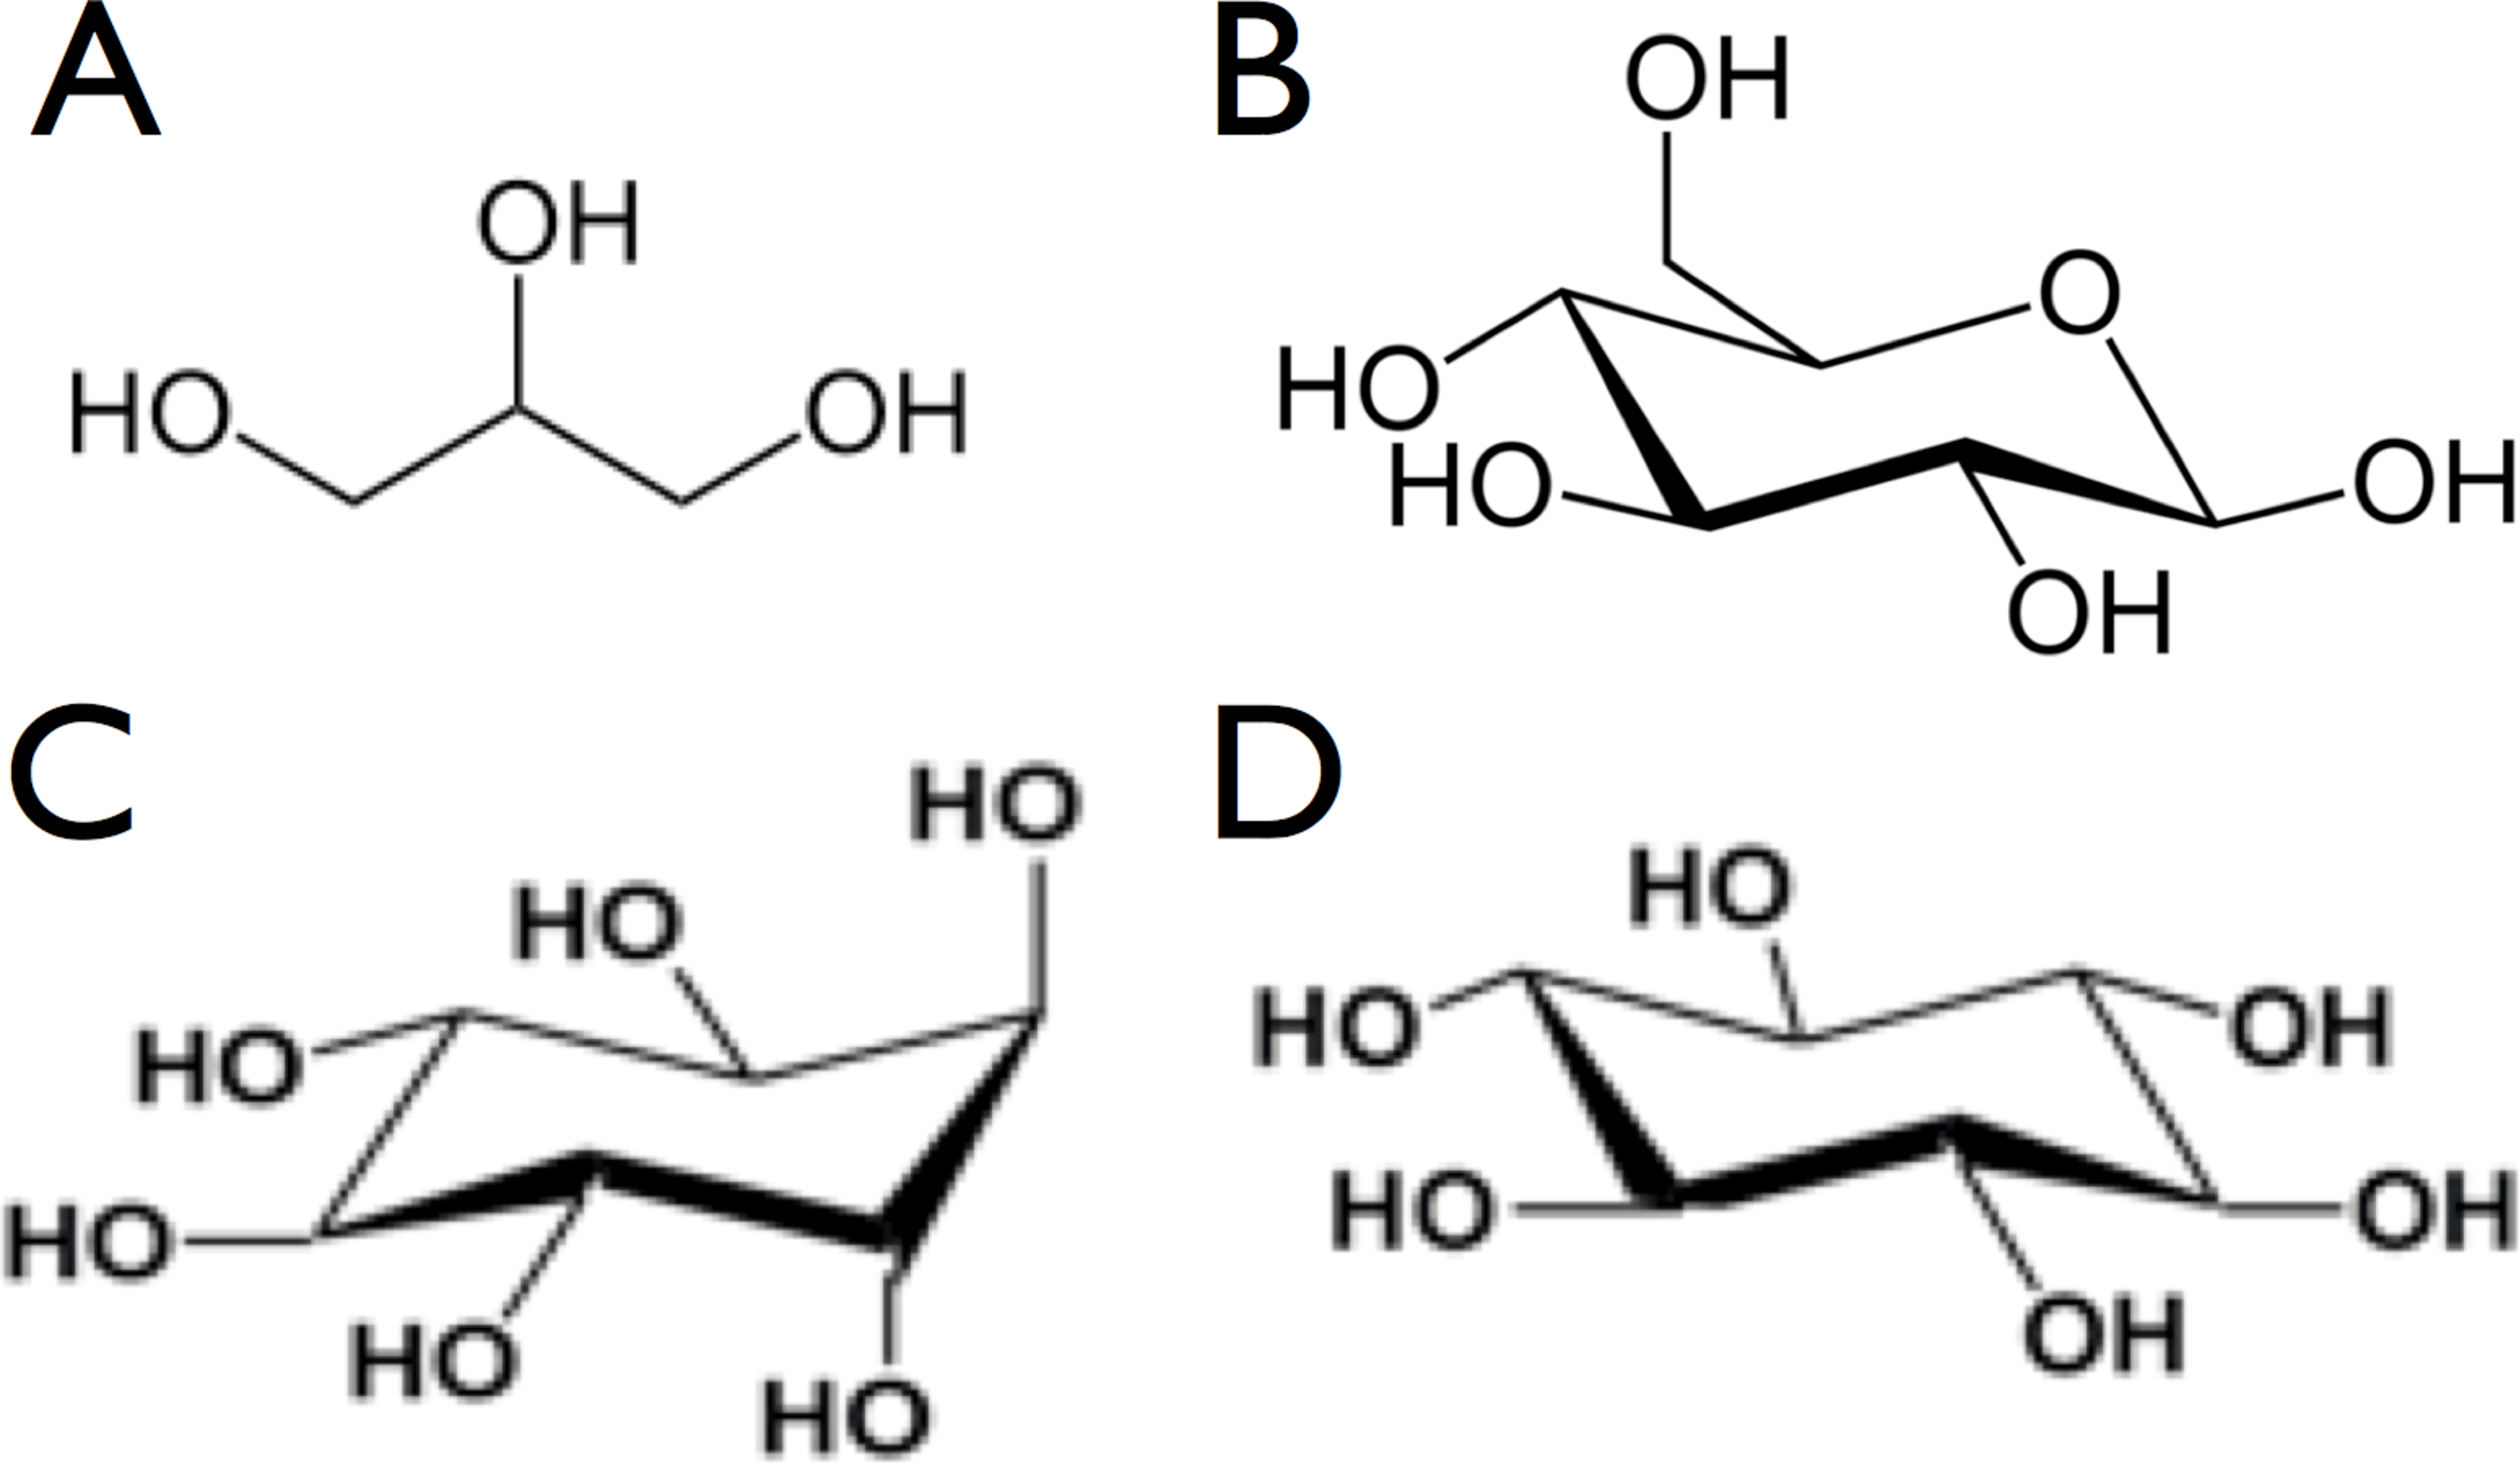
\includegraphics[width=2.5in]{figures/results3/ligands.pdf}
  \caption[Ligands]{Molecular structures of (A) glycerol, (B) glucose, (C) chiro-inositol and (D) scyllo-inositol}
  \label{fig:ligands}
\end{figure}

\begin{figure}[htbp]
  \centering
  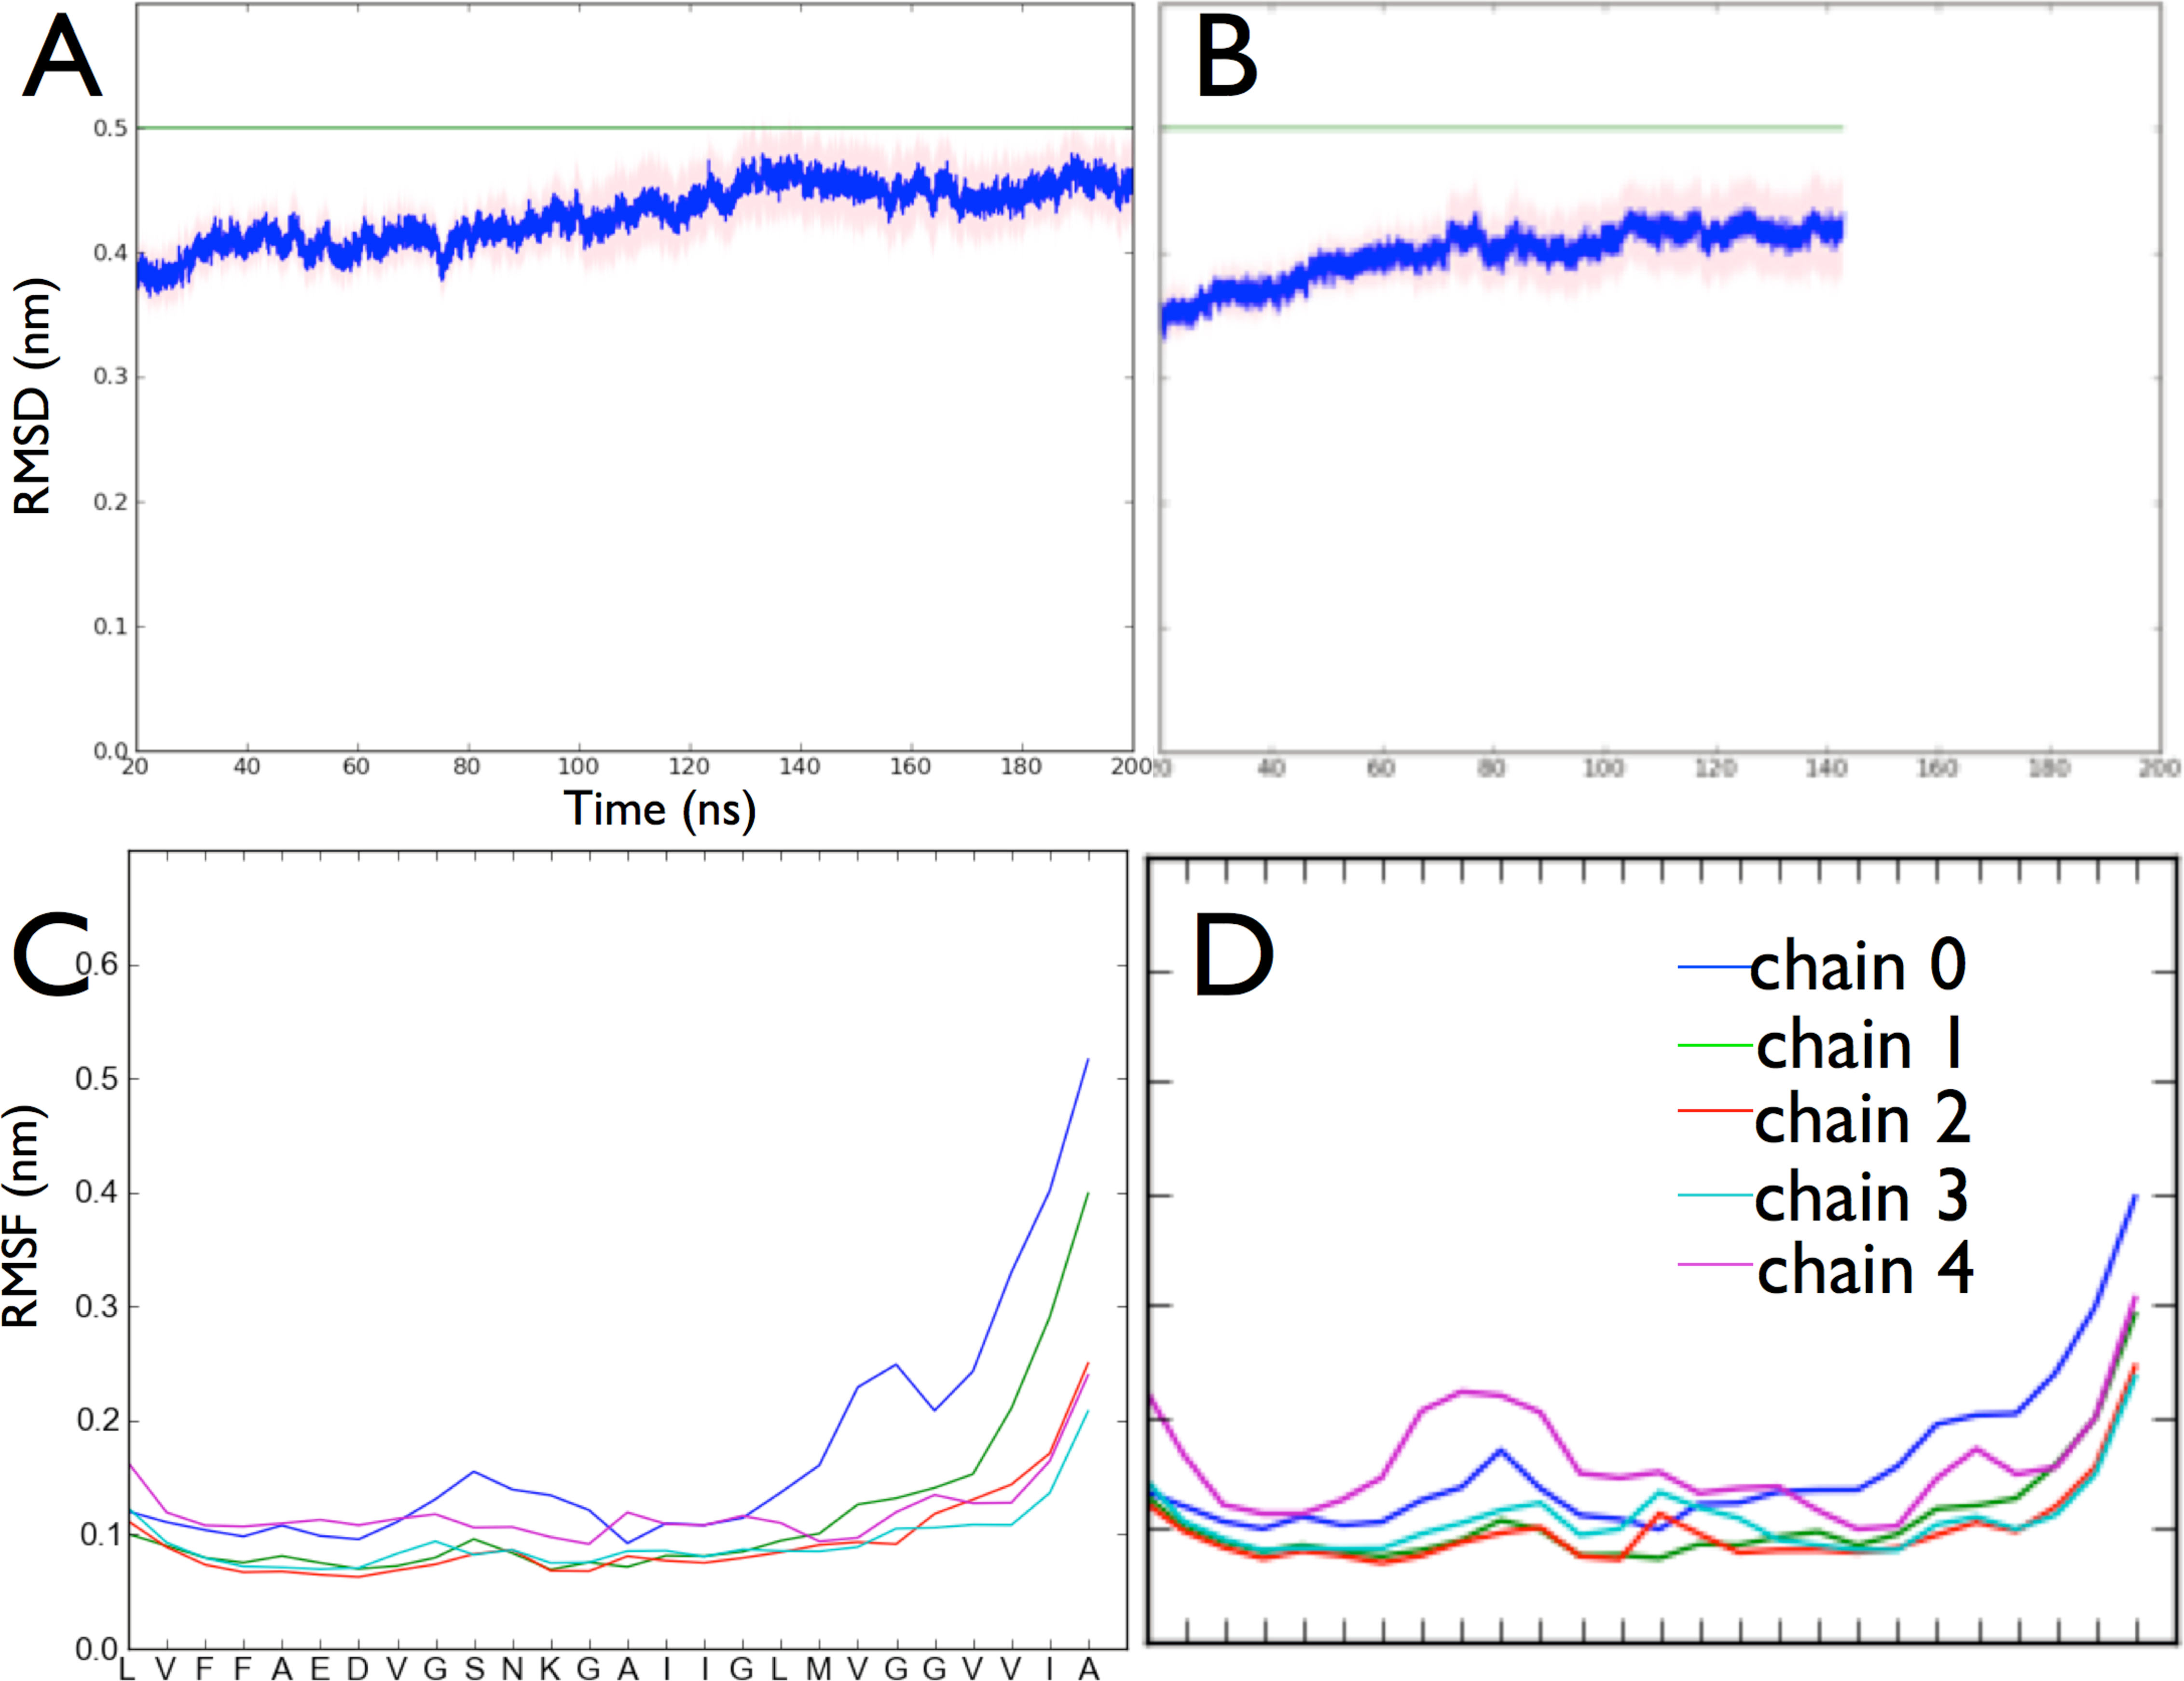
\includegraphics[width=5in]{figures/results3/protofibril_dynamics.pdf}
  \caption[RMSD and RMSF vs. time]{Fibril structure dynamics in pure water (A) and (C), and in the presence of scyllo-inositol (B) and (D).}
  \label{fig:protofibril_dynamics}
\end{figure}

\begin{figure}[htbp]
  \centering
  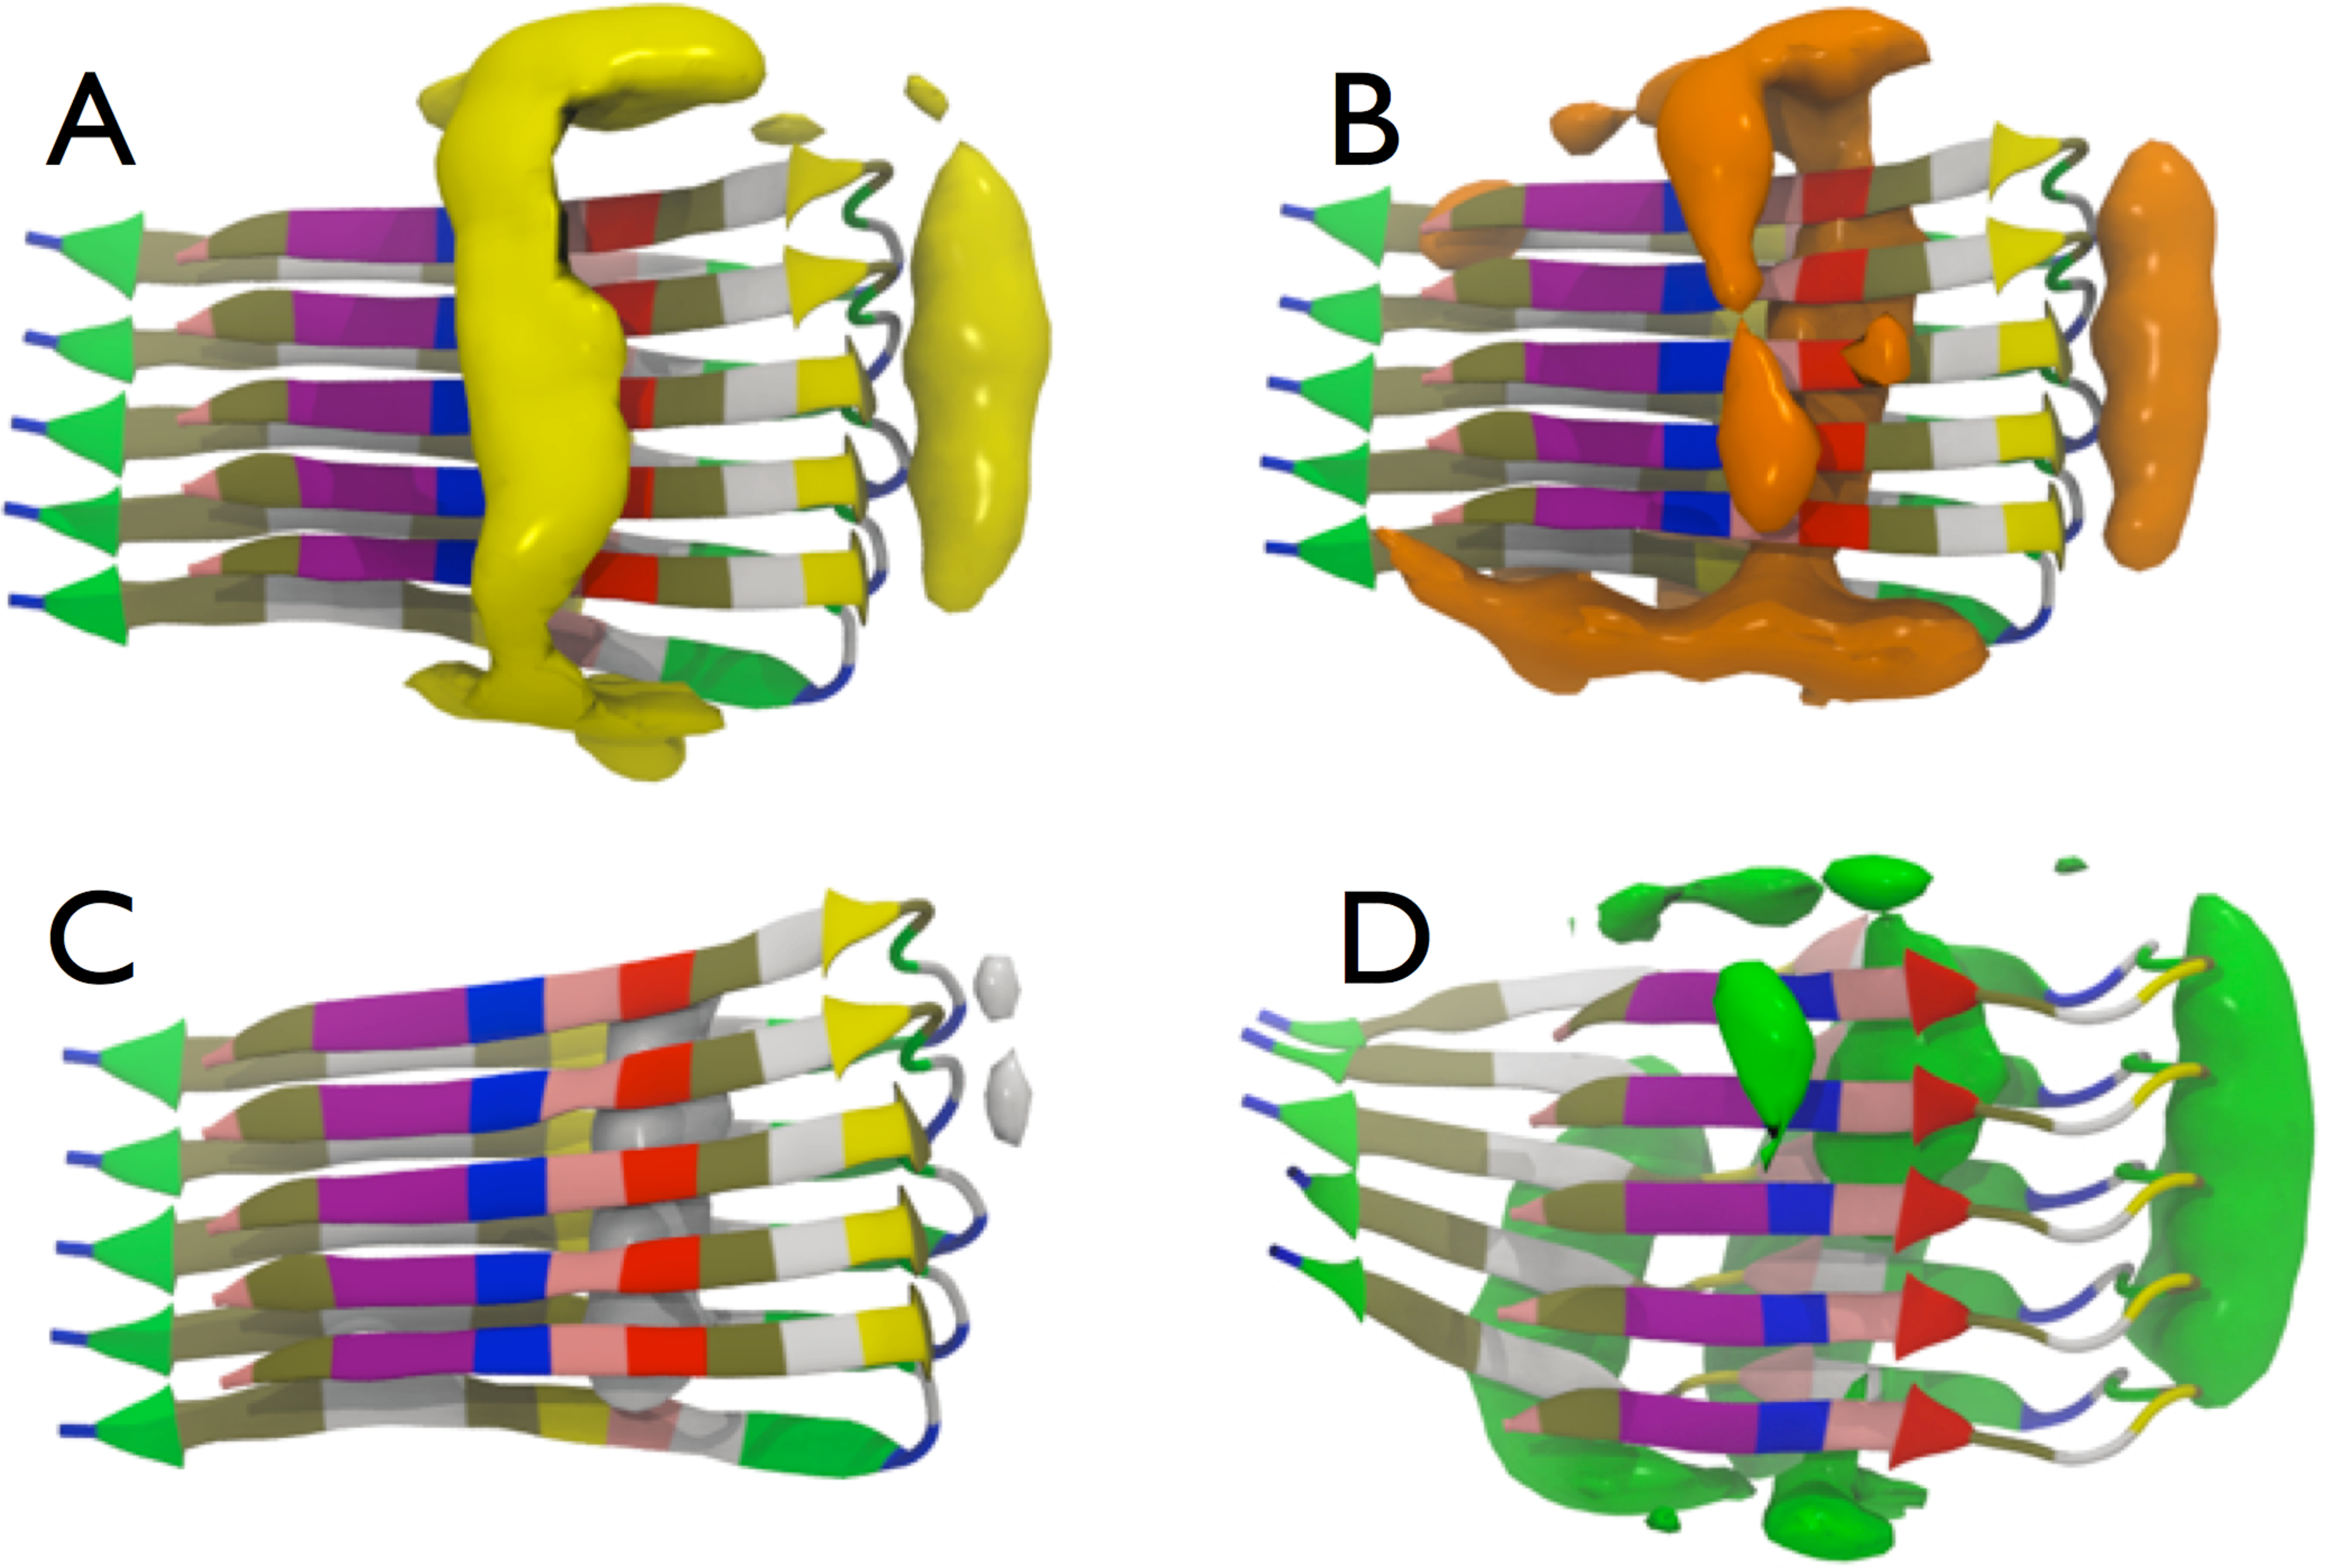
\includegraphics[width=6in]{figures/results3/binding_sdf.pdf}
  \caption[Abeta42 binding]{Comparisons of the spatial probability densities for (A) scyllo-inositol, (B) chiro-inositol (C) glycerol and (D) glucose.}
  \label{fig:spatial_binding}
\end{figure}

\begin{singlespace}
\addcontentsline{toc}{section}{Bibliography}
\bibliographystyle{elsart-num}
\bibliography{/Users/grace/github/thesis/document/results3/results3}
\end{singlespace}

